% Corazón v2 — artículo del proyecto final MIA-203 (Grupo 6). Compilar: latexmk -pdf main.tex
% Cada número viene de un archivo de results/ (indicado en un comentario junto a cada tabla).
\documentclass[conference]{IEEEtran}
\usepackage[utf8]{inputenc}
\usepackage[T1]{fontenc}
\usepackage[spanish,es-noshorthands,es-tabla,es-nodecimaldot]{babel}
\usepackage{amsmath,amssymb}
\usepackage{graphicx}
\usepackage{booktabs}
\usepackage{multirow}
\usepackage{xcolor}
\usepackage{tikz}
\usetikzlibrary{positioning,arrows.meta}
\usepackage[hidelinks]{hyperref}
\newcommand{\pendiente}[1]{\textcolor{red}{[PENDIENTE: #1]}}
\renewcommand{\IEEEkeywordsname}{Palabras clave}

\begin{document}

% Título: se decide al final entre los 3 candidatos (PLAN-DE-TRABAJO.md). Provisional:
%  1. Medir como el radiólogo: índice cardiotorácico por segmentación con U-Net frente a una CNN de caja negra para
%     detectar cardiomegalia
%  2. ¿Medir o clasificar? Índice cardiotorácico con U-Net frente a ResNet-50 en la detección de cardiomegalia en
%     radiografías de tórax
%  3. U-Net entrenada con máscaras automáticas para medir el índice cardiotorácico: comparación con una CNN de caja
%     negra y sesgo de la proyección AP
\title{Medir como el radiólogo: índice cardiotorácico por segmentación con U-Net frente a una CNN de caja negra para
detectar cardiomegalia}

\author{
\IEEEauthorblockN{Juan Sebastian Contreras Avendaño, Junior Francesco Romero Lovera, Luis Muñoz Cañabe,\\
Derly Raúl Oha Quispe, Lourdes Pedraza Palomino}
\IEEEauthorblockA{Grupo 6 · Maestría en Inteligencia Artificial, Facultad de Ingeniería Industrial y de Sistemas\\
Universidad Nacional de Ingeniería, Lima, Perú}
}

\maketitle

\begin{abstract}
La cardiomegalia se sospecha en la radiografía de tórax con el índice cardiotorácico (ICT), pero en gran parte del
Perú no hay un radiólogo que lo informe a tiempo. Comparamos dos formas de automatizarlo con aprendizaje profundo:
medir el ICT a partir de una U-Net que segmenta pulmones y corazón, entrenada con máscaras automáticas de CheXmask, o
clasificar con una ResNet-50 de caja negra. Usamos 8\,776 radiografías de ChestX-ray14 con partición por paciente y el
conjunto de prueba oficial (2\,354), tres semillas por modelo y contornos humanos (SCR, 147 placas) como referencia.
La U-Net midió el ICT con un acuerdo alto frente a los contornos humanos (ICC de 0.945 a 0.951; 0.964 a 0.971 tras
ajustarla con 80 placas humanas). Como detector, la ResNet-50 superó al ICT (AUC de 0.892 frente a 0.814). Ambos
métodos perdieron rendimiento en placas AP; en el ICT el sesgo se explica por la magnificación y una regresión
logística con la vista elevó la especificidad en AP de 0.356 a 0.619. En 300 fotos de 100 radiografías tomadas con dos
celulares, ambos perdieron de 0.02 a 0.03 de AUC, pero el ICT cambió de decisión en 4.7--8.3\,\% de las placas frente a
8.3--13.3\,\% de la ResNet-50. Medir no gana en exactitud, pero da una cifra que el médico puede ver, revisar y
corregir; la publicamos en una aplicación web que corre en el celular.
\end{abstract}

\begin{IEEEkeywords}
aprendizaje profundo, U-Net, índice cardiotorácico, cardiomegalia, radiografía de tórax, etiquetas débiles
\end{IEEEkeywords}

% ---------------------------------------------------------------------------------------------------------------------
\section{Introducción}

\pendiente{motivación peruana con cifras verificadas en su fuente: radiólogos fuera de Lima, corazón en la altura,
Telesalud (CONTEXTO-Y-ANTECEDENTES.md, §3; hoy POR CONFIRMAR).}

El ICT es el cociente entre el ancho máximo del corazón y el ancho interno del tórax; un valor mayor que 0.50 en una
placa posteroanterior (PA) sugiere cardiomegalia. Es una medida geométrica: si una red dibuja el corazón y los
pulmones, el ICT sale de esos contornos con una regla, igual que lo haría el radiólogo. La alternativa habitual es un
clasificador que entrega una probabilidad sin decir de dónde sale.

Este trabajo compara ambas familias del curso en el mismo problema y con las mismas particiones: segmentación con una
U-Net~\cite{ronneberger2015unet} y clasificación con una ResNet-50 preentrenada~\cite{he2016resnet}. La entrada es
una radiografía frontal de tórax; las salidas son el ICT (y sus componentes) o la probabilidad de cardiomegalia. El
éxito se mide en tres frentes: acuerdo con contornos humanos, capacidad de detección (AUC) y estabilidad ante dos
fuentes de error del mundo real: la proyección anteroposterior (AP), que agranda el corazón, y la radiografía que llega
como foto de celular.

Las contribuciones de este trabajo son:
\begin{itemize}
\item Una comparación controlada ``medir frente a clasificar'' en la que la U-Net se entrena con \emph{máscaras
  automáticas} (CheXmask) y se evalúa contra \emph{contornos humanos} (SCR).
\item La medición del atajo de la proyección AP en ChestX-ray14 para ambos enfoques, con una corrección explícita para
  el ICT y Grad-CAM para la caja negra.
\item Una prueba propia con 300 fotos de celular de 100 radiografías, con marcas fiduciales para enderezarlas, y una
  aplicación web que mide el ICT en el dispositivo y deja corregir la medida.
\end{itemize}

El resto del artículo se organiza así: la Sección~\ref{sec:rel} revisa trabajos relacionados; la
Sección~\ref{sec:met} describe la metodología; la Sección~\ref{sec:res} presenta los resultados, que se discuten en la
Sección~\ref{sec:dis}; la Sección~\ref{sec:con} concluye.

% ---------------------------------------------------------------------------------------------------------------------
\section{Trabajos relacionados}\label{sec:rel}

\textbf{Medir frente a clasificar la cardiomegalia.} Sogancioglu \emph{et al.}~\cite{sogancioglu2020cardiomegaly}
compararon en ChestX-ray14 un ICT calculado de una segmentación con un clasificador directo y encontraron ventaja para
la segmentación, entrenada con máscaras humanas. Chamveha \emph{et al.}~\cite{chamveha2020ctr} propusieron la
descomposición del ICT en las distancias de la línea media a cada borde del corazón, que usamos aquí. Nuestra
diferencia es entrenar la segmentación con máscaras automáticas a escala y medir, además, la robustez a la proyección
y a fotos.

\textbf{Arquitecturas base.} La U-Net~\cite{ronneberger2015unet} combina un codificador y un decodificador con
conexiones de salto y es el estándar de segmentación médica; la ResNet~\cite{he2016resnet} introdujo las conexiones
residuales y su versión preentrenada en ImageNet es una línea base habitual de clasificación. Grad-CAM~\cite{selvaraju2017gradcam}
pondera los mapas de la última capa convolucional por el gradiente de la clase para mostrar dónde mira la red.

\textbf{Datos y etiquetas.} ChestX-ray14~\cite{wang2017chestxray8} trae 112\,120 radiografías con etiquetas extraídas
de los informes. CheXmask~\cite{gaggion2024chexmask} publicó máscaras de pulmones y corazón generadas con un modelo,
con un índice de calidad por imagen (RCA). SCR~\cite{vanginneken2006scr} contiene contornos trazados por personas
sobre la base JSRT~\cite{shiraishi2000jsrt}, y es nuestra referencia dorada.

\textbf{Atajos y robustez.} Zech \emph{et al.}~\cite{zech2018confounding} mostraron que los modelos de radiografías
pueden aprender señales del hospital o del equipo en lugar de la enfermedad; la proyección AP, típica de pacientes en
cama, es una de esas señales. CheXphoto~\cite{phillips2020chexphoto} midió cuánto pierden los clasificadores con fotos
de radiografías, pero no evaluó medidas geométricas como el ICT.

% ---------------------------------------------------------------------------------------------------------------------
\section{Metodología}\label{sec:met}

\subsection{Datos}

\textbf{ChestX-ray14} (NIH Clinical Center~\cite{wang2017chestxray8}). Armamos un subconjunto con todas las placas
etiquetadas ``Cardiomegaly'' que tienen máscara en CheXmask y 6\,000 placas sin cardiomegalia (con o sin otros
hallazgos, no solo ``No Finding'', para que la red no aprenda ``sano frente a enfermo''). La prueba es la lista oficial
del NIH; entrenamiento y validación se separaron por \emph{Patient ID}, de modo que ningún paciente aparece en dos
particiones (Tabla~\ref{tab:datos}). En el subconjunto, el 43.7\,\% de las placas con cardiomegalia son AP frente al
38.5\,\% de las sin cardiomegalia: la vista está asociada a la etiqueta.

% results/kaggle-v2/runs/E1b_debil_rca07_s1/ict_unet.csv (split, cardio, view)
\begin{table}[t]
\caption{Resumen del conjunto de datos (ChestX-ray14, 5\,674 pacientes)}\label{tab:datos}
\centering
\begin{tabular}{lrrrr}
\toprule
Partición & Placas & Con cardiomegalia & Sin & AP \\
\midrule
Entrenamiento & 5\,416 & 1\,471 & 3\,945 & 1\,829 \\
Validación    & 1\,006 &   236 &   770 &   357 \\
Prueba (oficial) & 2\,354 & 1\,069 & 1\,285 & 1\,335 \\
\bottomrule
\end{tabular}
\end{table}

\textbf{Máscaras débiles: CheXmask}~\cite{gaggion2024chexmask} (CC BY 4.0). Decodificamos las máscaras de pulmón
derecho, pulmón izquierdo y corazón de las 8\,776 placas; 8\,666 tienen RCA $\geq 0.7$.

\textbf{Contornos humanos: SCR}~\cite{vanginneken2006scr} (CC BY 4.0) sobre 247 radiografías JSRT~\cite{shiraishi2000jsrt}.
Rasterizamos los contornos a máscaras. Usamos 147 placas como prueba dorada y 100 para el ajuste fino de E1c (80 para
entrenar y 20 para elegir la época).

\textbf{Preprocesamiento y aumento.} Todas las imágenes se llevan a gris de $256\times256$ píxeles con reducción por
área y se normalizan como $(x/255-0.5)/0.25$. En entrenamiento se aplican rotación de $\pm10^\circ$, escala de 0.9 a
1.1, traslación de $\pm5$\,\% y brillo y contraste de $\pm15$\,\%. No se voltea la imagen: el corazón está a la
izquierda del paciente y el volteo crearía anatomía falsa.

\textbf{Fotos con celular (E5).} Elegimos 100 placas de la prueba oficial, 25 por grupo (PA o AP, con o sin
cardiomegalia), y las mostramos en un monitor de $1920\times1080$ dentro de una lámina con cuatro marcas ArUco en las
esquinas y una quinta que codifica el número de placa~\cite{garrido2014aruco}. Se tomaron 300 fotos: iPhone~16~Pro de
frente y con inclinación, y Honor~X8b (LLY-LX3) de frente. Cada foto se endereza con una homografía estimada con las
esquinas de las marcas visibles (al menos 2 marcas, 8 puntos) y se recorta la radiografía. Como respaldo, se aplicaron
seis degradaciones sintéticas a las mismas placas: perspectiva, rotación de $7^\circ$, desenfoque, brillo, moiré y
compresión JPEG.

\subsection{Arquitecturas}

La Fig.~\ref{fig:pipeline} resume el sistema.

\begin{figure}[t]
\centering
\resizebox{\linewidth}{!}{\begin{tikzpicture}[font=\scriptsize, node distance=3mm and 4mm,
  caja/.style={draw, rounded corners=2pt, align=center, inner sep=3pt, minimum height=8mm},
  flecha/.style={-{Stealth[length=2mm]}}]
\node[caja] (x) {Radiografía\\$1\times256\times256$};
\node[caja, right=of x, yshift=6mm] (u) {U-Net\\7.8\,M parám.};
\node[caja, right=of u] (m) {Máscaras\\$3\times256\times256$};
\node[caja, right=of m] (ict) {MRD, MLD, ID\\$\Rightarrow$ ICT};
\node[caja, right=of x, yshift=-6mm] (r) {ResNet-50\\23.5\,M parám.};
\node[caja, right=of r] (p) {$p$(cardiomegalia)};
\node[caja, right=of p] (g) {Grad-CAM};
\draw[flecha] (x) -- (u); \draw[flecha] (u) -- (m); \draw[flecha] (m) -- (ict);
\draw[flecha] (x) -- (r); \draw[flecha] (r) -- (p); \draw[flecha] (p) -- (g);
\end{tikzpicture}}
\caption{Dos caminos para la misma radiografía: medir el ICT a partir de los contornos (arriba) o clasificar con una
caja negra (abajo).}\label{fig:pipeline}
\end{figure}

\textbf{U-Net} implementada desde cero (reutilizada del examen parcial del grupo). Tiene cuatro niveles de
submuestreo con 32, 64, 128 y 256 canales y un cuello de botella de 512. Cada bloque aplica dos veces convolución
$3\times3$ con relleno, \emph{BatchNorm} y ReLU. Sube con convolución transpuesta $2\times2$ y concatena el salto; cierra
con una convolución $1\times1$ que da 3 canales: pulmón derecho, pulmón izquierdo y corazón. Cada canal lleva su propia
sigmoide, porque el corazón se superpone a los pulmones y las clases no son excluyentes. Tiene 7.76\,M de parámetros,
todos entrenados.

\textbf{ResNet-50}~\cite{he2016resnet} preentrenada en ImageNet, con la capa final cambiada por una salida única. La
radiografía en gris se repite en tres canales y se normaliza como ImageNet. Usa las mismas imágenes de 256 píxeles, la
misma partición y el mismo aumento que la U-Net. Tiene 23.5\,M de parámetros, todos ajustados.

\subsection{Formulación y función de pérdida}

\textbf{Segmentación.} Sea $\hat{y}_{c,i}=\sigma(z_{c,i})$ la probabilidad del píxel $i$ en el canal
$c\in\{1,2,3\}$ y $y_{c,i}\in\{0,1\}$ la máscara. La pérdida combina entropía cruzada binaria y Dice por canal:
\begin{equation}
\mathcal{L}_{\text{seg}} = \text{BCE}(\hat{y},y) + 1 - \frac{1}{3}\sum_{c=1}^{3}
\frac{2\sum_i \hat{y}_{c,i}y_{c,i}+\epsilon}{\sum_i \hat{y}_{c,i}+\sum_i y_{c,i}+\epsilon},
\end{equation}
con $\epsilon=1$. El Dice se promedia por canal para que los pulmones, más grandes, no dominen al corazón.

\textbf{Índice cardiotorácico.} Binarizamos cada canal en 0.5 y conservamos su mayor componente conexa. El diámetro
interno del tórax ID es la fila con mayor distancia entre el borde externo del pulmón derecho y el del pulmón
izquierdo; su punto medio define la línea media $x_m$. Con $x_{\min}$ y $x_{\max}$, los bordes del corazón,
\begin{gather}
\text{MRD}=\max(0,x_m-x_{\min}),\ \ \text{MLD}=\max(0,x_{\max}-x_m),\\
\text{ICT}=\frac{\text{MRD}+\text{MLD}}{\text{ID}}.
\end{gather}
Si falta alguna estructura, la placa se declara no medible. Con el tamaño de píxel del NIH, MRD se expresa también en
centímetros.

\textbf{Clasificación.} Entropía cruzada binaria con peso para la clase positiva
$w_+=N_-/N_+$, calculado en entrenamiento (27\,\% de cardiomegalia):
\begin{equation}
\mathcal{L}_{\text{cls}} = -\frac{1}{N}\sum_{n=1}^{N}\left[w_+\,y_n\log p_n + (1-y_n)\log(1-p_n)\right].
\end{equation}

\textbf{Grad-CAM}~\cite{selvaraju2017gradcam} sobre la última etapa convolucional (\texttt{layer4}). Por placa
calculamos la energía del mapa dentro del corazón, $E=\sum_i M_i\,h_i/\sum_i M_i$ ($h$ = máscara del corazón), y la
dividimos por el área del corazón. Una razón de 1 equivale a un mapa uniforme.

\subsection{Experimentos}

\begin{itemize}
\item \textbf{E1, segmentación:} máscaras débiles completas (E1a) frente a filtradas por RCA $\geq0.7$ (E1b) y E1b
  ajustada con 80 placas humanas (E1c). Se mide el Dice en la prueba dorada SCR.
\item \textbf{E2, diagnóstico:} AUC del ICT (U-Net), de la ResNet-50 y de dos líneas base: el ICT calculado
  directamente de las máscaras de CheXmask (sin red) y una regresión logística sobre [ICT, vista AP] ajustada en
  entrenamiento.
\item \textbf{E3, acuerdo clínico:} ICT de la U-Net frente al ICT de los contornos humanos en SCR, con ICC(A,1)
  de McGraw y Wong~\cite{mcgraw1996icc} y límites de Bland-Altman~\cite{bland1986agreement}.
\item \textbf{E4, proyección:} AUC por vista; una ResNet-50 entrenada solo con placas PA; la ``fuga de vista'', que es
  el AUC del puntaje para separar AP de PA \emph{solo entre placas sin cardiomegalia} (0.5 = el puntaje no codifica la
  vista); y Grad-CAM.
\item \textbf{E5, fotos:} para cada foto y cada semilla, cambio del ICT y de la probabilidad frente a la placa original,
  porcentaje de decisiones que cambian y AUC. La comparación entre la foto enderezada y la recortada sin enderezar usa
  las mismas placas.
\item \textbf{E6, lado derecho:} AUC de MRD/ID y de MLD/ID por separado, y su distribución en aciertos y errores del
  ICT.
\end{itemize}

\subsection{Entrenamiento y métricas}

Ambos modelos usan AdamW~\cite{loshchilov2019adamw} con decaimiento de pesos $10^{-4}$, tasa de aprendizaje con
política de un ciclo (\emph{OneCycle}) y precisión mixta. La U-Net entrena 30 épocas con lote de 16 y tasa máxima de
$10^{-3}$; el ajuste E1c, 30 épocas con lote de 8 y $2\times10^{-4}$. La ResNet-50 entrena 12 épocas con lote de 32 y
$3\times10^{-4}$. La época se elige en validación: el Dice medio con máscaras débiles (U-Net), el Dice en las 20 placas
humanas reservadas (E1c) o el AUC (ResNet). El umbral de la ResNet es el de Youden~\cite{youden1950index} en
validación; el del ICT es el clínico de 0.50, sin ajustar. La prueba no se usó para elegir nada. Cada experimento se
repite con las semillas 0, 1 y 2 y se reporta media $\pm$ desviación estándar. Reportamos AUC, sensibilidad,
especificidad y F1, porque la prueba no está balanceada (45\,\% de cardiomegalia).

\textbf{Hardware.} Kaggle con dos GPU Tesla T4. El primer día entrenamos 62.6~min (dos U-Net y el ajuste). El segundo
día, 150.6~min de U-Net y 38.2~min de ResNet-50 con Grad-CAM, en paralelo. En total fueron unas 4.2~horas de GPU. E5 y E6
corrieron en el CPU de una laptop: E5 tardó 35.5~min para 6 modelos y 13 condiciones de 73 a 100 placas.

% ---------------------------------------------------------------------------------------------------------------------
\section{Resultados}\label{sec:res}

\subsection{Comparación con las líneas base}

% results/kaggle-v2/E2_diagnostico.csv
\begin{table}[t]
\caption{Detección de cardiomegalia en la prueba oficial (2\,354 placas; media $\pm$ D.\,E., 3 semillas)}\label{tab:e2}
\centering
\setlength{\tabcolsep}{4pt}
\begin{tabular}{lcccc}
\toprule
Método & AUC & Sens. & Esp. & F1 \\
\midrule
ResNet-50 (PA + AP) & \textbf{0.892 $\pm$ 0.010} & 0.830 & \textbf{0.786} & \textbf{0.795} \\
ResNet-50 (solo PA) & 0.865 $\pm$ 0.014 & 0.771 & 0.783 & 0.759 \\
ICT, U-Net E1b & 0.814 $\pm$ 0.001 & 0.925 & 0.488 & 0.728 \\
ICT + vista (reg. log.) & 0.810 $\pm$ 0.001 & 0.834 & 0.615 & 0.726 \\
ICT, CheXmask (sin red) & 0.801 & 0.930 & 0.471 & 0.725 \\
ICT, U-Net E1c & 0.796 $\pm$ 0.006 & \textbf{0.955} & 0.407 & 0.716 \\
\bottomrule
\end{tabular}
\\[2pt]{\footnotesize Sensibilidad, especificidad y F1 al umbral de Youden en validación. ICT al umbral clínico de
0.50: sensibilidad 0.918, especificidad 0.504.}
\end{table}

La ResNet-50 detecta mejor que el ICT (Tabla~\ref{tab:e2}). El ICT de la U-Net supera al calculado directamente de
CheXmask (0.814 frente a 0.801), y la U-Net ajustada con contornos humanos, que mide mejor (Tabla~\ref{tab:e1}),
diagnostica peor (0.796).

\subsection{Segmentación, acuerdo clínico y ablación de las etiquetas}

% results/kaggle-v2/LEEME.md (E1, E3) y E3_acuerdo_ict.csv
\begin{table}[t]
\caption{Segmentación y acuerdo del ICT en la prueba dorada SCR (147 placas; 3 semillas)}\label{tab:e1}
\centering
\setlength{\tabcolsep}{3pt}
\resizebox{\linewidth}{!}{\begin{tabular}{lcccc}
\toprule
Variante & Dice corazón & Dice medio & Error ICT & ICC(A,1) \\
\midrule
E1a débil, todas & 0.936 $\pm$ 0.001 & 0.962 $\pm$ 0.001 & 0.012 & 0.948--0.953 \\
E1b débil, RCA $\geq$ 0.7 & 0.936 $\pm$ 0.001 & 0.961 $\pm$ 0.001 & 0.012 & 0.945--0.951 \\
E1c E1b + 80 humanas & \textbf{0.951 $\pm$ 0.001} & \textbf{0.971 $\pm$ 0.000} & \textbf{0.010} & \textbf{0.964--0.971} \\
\bottomrule
\end{tabular}}
\\[2pt]{\footnotesize Error ICT = error absoluto medio frente al ICT de los contornos humanos. ICC: rango entre semillas.}
\end{table}

Filtrar CheXmask por calidad no cambió nada medible: solo 110 de 8\,776 máscaras quedan por debajo de RCA 0.7. El
ajuste con 80 placas humanas subió el Dice del corazón de 0.936 a 0.951 y el ICC a 0.964--0.971. En E1c, el sesgo del
ICT frente a los humanos está entre $-0.0035$ y $-0.0005$ y los límites de Bland-Altman son de alrededor de
$\pm0.03$. En las tres variantes, la decisión ICT $\geq 0.50$ coincide con la de los contornos humanos en el
93--96\,\% de las placas.

\subsection{Proyección AP e interpretabilidad}

% results/kaggle-v2/E4_por_vista.csv
\begin{table}[t]
\caption{Efecto de la proyección (prueba oficial: 1\,019 PA, 1\,335 AP)}\label{tab:e4}
\centering
\setlength{\tabcolsep}{4pt}
\begin{tabular}{lcccc}
\toprule
Método & AUC PA & AUC AP & Esp. AP & Fuga de vista \\
\midrule
ResNet-50 (PA + AP) & 0.944 & 0.845 & 0.750 & 0.646 $\pm$ 0.055 \\
ResNet-50 (solo PA) & 0.936 & 0.795 & 0.731 & 0.710 $\pm$ 0.045 \\
ICT, U-Net & 0.864 & 0.776 & 0.356 & 0.691 $\pm$ 0.011 \\
ICT + vista & 0.864 & 0.776 & 0.619 & \textbf{0.493 $\pm$ 0.011} \\
\bottomrule
\end{tabular}
\\[2pt]{\footnotesize Esp. AP al umbral de Youden. Fuga de vista: AUC para separar AP de PA entre placas sin
cardiomegalia; 0.5 = no codifica la vista.}
\end{table}

Todos los métodos rinden menos en AP (Tabla~\ref{tab:e4}). En el ICT, la especificidad en AP cae a 0.356: la
magnificación hace que muchos corazones normales pasen de 0.50. Como la causa es conocida, se corrige con la vista; la
regresión logística baja la fuga a 0.493 y sube la especificidad en AP a 0.619. La ResNet-50 entrenada solo con PA
pierde 0.141 de AUC al pasar a AP, frente a 0.099 de la entrenada con ambas vistas.

Cuando la ResNet-50 predice ``cardiomegalia'', la energía de Grad-CAM dentro del corazón es de 4.3 a 6.4 veces la que
tendría un mapa uniforme, acierte o no. En los negativos correctos, la razón baja a 1.2--4.3 (rangos entre corridas y
vistas). La Fig.~\ref{fig:gradcam} muestra ejemplos; en uno se ve el rótulo ``PORTABLE'', una pista de la vista AP
que está a la vista de la red. \pendiente{análisis fino de Grad-CAM por acierto y vista.}

\begin{figure}[t]
\centering
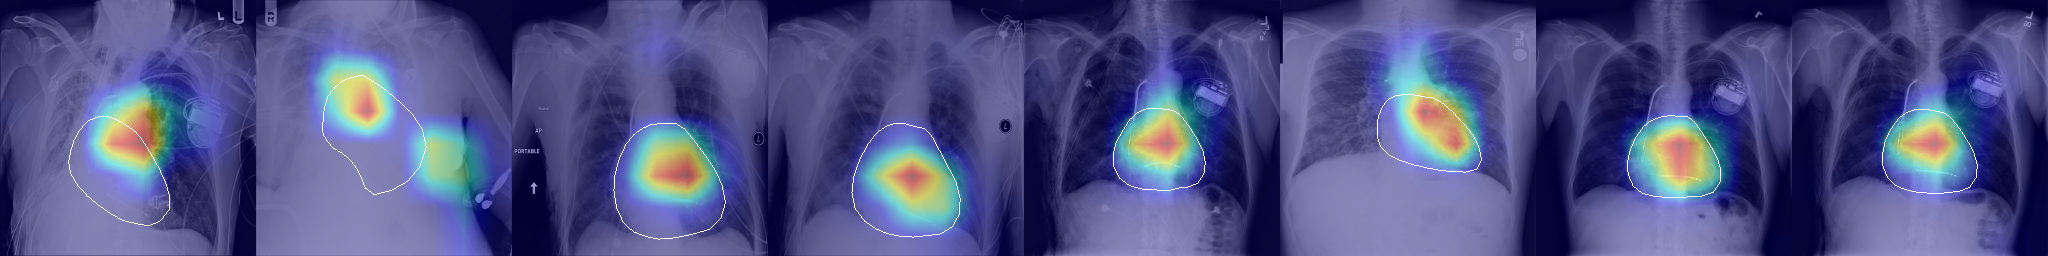
\includegraphics[width=\linewidth]{figs/gradcam.png}
\caption{Grad-CAM de la ResNet-50 (semilla 0) en placas de prueba; contorno blanco: corazón de CheXmask.}\label{fig:gradcam}
\end{figure}

\subsection{Fotos con celular}

% results/e5/E5_resumen.csv y E5_pareado_sin_corregir.csv
\begin{table}[t]
\caption{Fotos con celular: 100 placas, 3 semillas por modelo (media $\pm$ D.\,E.)}\label{tab:e5}
\centering
\setlength{\tabcolsep}{3pt}
\begin{tabular}{lcccc}
\toprule
& \multicolumn{2}{c}{ICT (U-Net)} & \multicolumn{2}{c}{ResNet-50} \\
Condición & AUC & Cambia & AUC & Cambia \\
\midrule
Original & 0.827 $\pm$ 0.008 & -- & 0.899 $\pm$ 0.020 & -- \\
iPhone, frente & 0.801 $\pm$ 0.009 & 6.7\,\% & 0.872 $\pm$ 0.020 & 13.3\,\% \\
iPhone, inclinada & 0.797 $\pm$ 0.014 & 8.3\,\% & 0.883 $\pm$ 0.010 & 10.3\,\% \\
Honor, frente & 0.812 $\pm$ 0.014 & 4.7\,\% & 0.881 $\pm$ 0.011 & 8.3\,\% \\
Sintéticas (6) & 0.814--0.833 & 2.0--5.3\,\% & 0.891--0.908 & 4.3--22.3\,\% \\
\bottomrule
\end{tabular}
\\[2pt]{\footnotesize ``Cambia'': placas cuya decisión (ICT 0.50; ResNet, umbral de Youden) difiere de la original.}
\end{table}

Se leyeron todas las fotos (301; una placa se fotografió dos veces con el Honor) y las 100 placas quedaron cubiertas
con cada celular (Tabla~\ref{tab:e5}). Ambos métodos
pierden entre 0.02 y 0.03 de AUC. El ICT cambia de decisión en menos placas que la ResNet-50, y lo hace en casos
limítrofes: las 59 mediciones de 899 que cruzan el umbral estaban a una mediana de 0.013 de 0.50, frente a 0.056 en
todas. El cambio absoluto mediano del ICT fue de 0.010 a 0.012. Sobre las mismas placas, enderezar la foto aportó poco
(ICT: 5.9 frente a 8.2\,\% de decisiones que cambian con el Honor; 10.3 frente a 10.7\,\% con el iPhone inclinado);
la inclinación lograda fue moderada. Las degradaciones sintéticas subestimaron el efecto real sobre el ICT.

\subsection{El lado derecho del corazón}

% results/e6/E6_auc_componentes.csv, E6_aciertos_errores.csv, E6_fn_mrd_alto.csv
Por separado, MLD/ID tiene un AUC de 0.735 $\pm$ 0.003 y MRD/ID uno de 0.697 $\pm$ 0.003; su suma (el ICT) da 0.814.
Los falsos negativos del ICT no esconden un lado derecho grande: su MRD/ID mediano (0.138--0.154) se parece al de los
verdaderos negativos (0.137--0.148) y está lejos del de los verdaderos positivos (0.188--0.204). Solo el 13--16\,\% de
los falsos negativos supera el percentil 90 de los verdaderos negativos. En los cuatro grupos, MRD en centímetros es
mayor en AP que en PA (p.\,ej., 4.59 frente a 4.18~cm en los verdaderos negativos).

\subsection{Aplicación y costo de inferencia}

La U-Net se exportó a ONNX (31~MB) y se verificó contra PyTorch: la diferencia máxima de probabilidad fue de
$2.5\times10^{-6}$ y el 100\,\% de los píxeles coincidió. La aplicación web corre en el navegador sin enviar la
imagen (Fig.~\ref{fig:app}). En una laptop, una medición tarda de 1.7 a 3.2~s. Para una foto, el usuario marca las
cuatro esquinas de la radiografía; las líneas de la medida se pueden arrastrar para corregirla. En dos ejemplos y en
una foto real da el mismo ICT que el código de Python.

\begin{figure}[t]
\centering
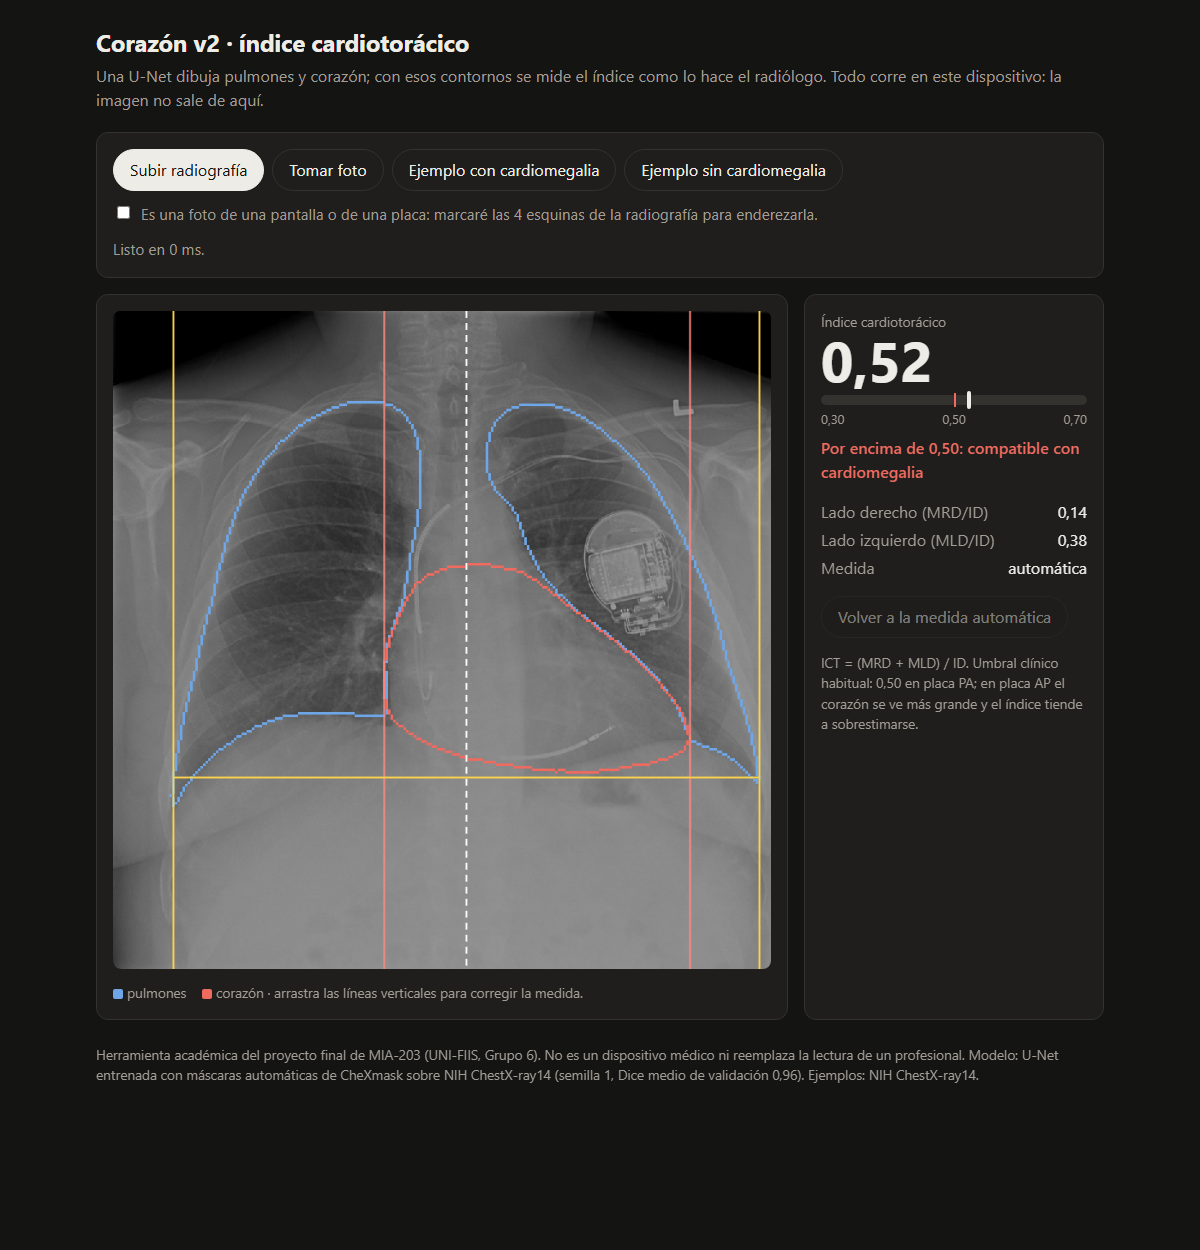
\includegraphics[width=\linewidth]{figs/app.png}
\caption{Aplicación web: contornos de la U-Net, línea media, bordes del corazón y del tórax, e ICT.}\label{fig:app}
\end{figure}

% ---------------------------------------------------------------------------------------------------------------------
\section{Discusión}\label{sec:dis}

\pendiente{redactar el viernes. Puntos acordados a partir de los resultados:}
\begin{itemize}
\item H2 se refuta: la caja negra detecta mejor (0.892 frente a 0.814). A diferencia
  de~\cite{sogancioglu2020cardiomegaly}, nuestra segmentación se entrenó con máscaras automáticas y el umbral 0.50 no
  es necesariamente el criterio de los informes del NIH. Que E1c mida mejor y diagnostique peor apoya esta lectura
  (POR CONFIRMAR).
\item El valor del ICT está en que se puede auditar: su error en AP tiene causa conocida y corrección, y en las fotos
  solo cambia de decisión en casos limítrofes.
\item La ResNet-50 aprende la vista (fuga de 0.646 a 0.710) y puede usar rótulos como ``PORTABLE''.
\item Limitaciones: etiquetas del NIH extraídas por procesamiento de lenguaje; población de EE.\,UU. y Japón; umbral
  0.50 de poblaciones de llanura; las fotos son de una pantalla y no de placas físicas; una sola sesión de fotos; el
  ICT no aísla el ventrículo derecho. No es un dispositivo médico.
\end{itemize}

\section{Conclusiones}\label{sec:con}

\pendiente{redactar el viernes, 1--2 párrafos sin repetir el resumen, con trabajo futuro concreto.}

\section*{Contribuciones}

\pendiente{tareas de cada integrante; las define el equipo.}

\begin{center}
\begin{tabular}{p{0.38\linewidth}p{0.52\linewidth}}
\toprule
Integrante & Tareas en las que participó \\
\midrule
Juan Sebastian Contreras Avendaño & \pendiente{} \\
Junior Francesco Romero Lovera & \pendiente{} \\
Luis Muñoz Cañabe & \pendiente{} \\
Derly Raúl Oha Quispe & \pendiente{} \\
Lourdes Pedraza Palomino & \pendiente{} \\
\bottomrule
\end{tabular}
\end{center}

\section*{Disponibilidad de código y uso de herramientas de IA}

Código, resultados y aplicación: \url{https://github.com/loupv99/corazon-v2}. Pesos: \pendiente{enlace a los pesos}.
\pendiente{declaración de uso de asistentes de IA (qué herramienta y para qué); la redacta el equipo.}

\bibliographystyle{IEEEtran}
\bibliography{refs}

\end{document}
